\documentclass[UTF8]{ctexbook}
\usepackage{tikz}
\usetikzlibrary{arrows.meta}
\usepackage[siunitx]{circuitikz}
\usepackage{graphicx}
\usepackage{wrapfig}
\usepackage{enumitem}
\usepackage{amsmath,amssymb}
\usepackage{xcolor}
\usepackage{geometry}
\geometry{a4paper,margin=2.5cm}
\sisetup{inter-unit-product = \ensuremath{{}\cdot{}}}
\definecolor{elecblue}{RGB}{0,155,220} % 电路图用的蓝色
\begin{document}
\setcounter{chapter}{1}
\chapter{Circuit Elements}
\section{理想电源:电压源与电流源}
\subsection{电源的物理意义}
\paragraph*{电源}:能在两端保持一定电压或电流、并在电能与其他形式能量之间进行转换的装置。
\begin{itemize}
\item 电源既可以\textbf{向电路输送功率}(发电),也可以\textbf{从电路吸收功率}(充电、制动等)。
\end{itemize}
\paragraph*{理想独立源:}是指能够提供与其他电路元件完全无关的特定电压或电流的有源元件。
\paragraph*{受控源(理想非独立源):}是指其所提供的电压或电流受到其他电压或电流控制的有源元件。
\subsection{理想独立电压源}
\begin{description}[leftmargin=37pt,labelsep=0.5em]
\item[定义:]
在一个两端口元件上,端电压被规定为某个给定函数 $v_s(t)$,并且与通过该元件的电流 $i(t)$ 无关的理想元件。
\end{description}
\begin{itemize}
\item (a)用于表示恒定电压或时变电压
\item (b)用于表示恒定电压
\end{itemize}
\noindent\textbf{理想电压模型}:端电压恒定为指定值$v_s$,不随负载电流变化:
\[v = v_s \quad\text{(纵轴为 $v$,为一条水平线)}\]
\begin{figure}[htbp]
\centering
  %============== 左:两个独立电压源符号 ==================
\begin{minipage}[c]{0.1\textwidth}
\centering
\begin{tikzpicture}[line cap=round,line join=round,x=0.7cm,y=0.7cm]
% 颜色与样式
\definecolor{wireblue}{RGB}{0,90,150}
\definecolor{termred}{RGB}{190,30,30}
\definecolor{srcyellow}{RGB}{255,230,160}
\definecolor{srcgreen}{RGB}{0,140,90}
\tikzset{wire/.style={draw=wireblue,line width=1.4pt},term/.style={draw=termred,line width=1.4pt},src/.style={draw=termred,line width=1.4pt,fill=srcyellow}}
%---------------- 左边:电压源 ----------------
 % 导线
\draw[wire] (0,0) -- (0,4);
\draw[wire] (0,4) -- (3,4);
\draw[wire] (0,0) -- (3,0);
% 右侧端点
\draw[term] (3,4) -- (3.4,4);
\draw[term] (3.4,4) circle (0.13);
\draw[term] (3,0) -- (3.4,0);
\draw[term] (3.4,0) circle (0.13);
% 圆形电压源
\draw[src] (0,2) circle (0.4);
% 圆内 + 号和 - 号
\draw[term,line width=0.9pt] (-0.15,2.15) -- (0.15,2.15); % +
\draw[term,line width=0.9pt] (0,2) -- (0,2.3);
\draw[term,line width=0.9pt] (-0.15,1.8) -- (0.15,1.8);   % -
% v 标注
\node[left,font=\Large] at (-0.4,2) {$v$};
\node at (2,-1.35) {$(a)$};
%---------------- 右边:理想电压源 V ----------------
\begin{scope}[xshift=4cm]  % 整个右图平移
% 导线:下面一段 + 上面一段,中间留给电源符号
\draw[wire] (0,0) -- (0,2);
\draw[wire] (0,2.3) -- (0,4);
\draw[wire] (0,4) -- (3,4);
\draw[wire] (0,0) -- (3,0);
% 右侧端点
\draw[term] (3,4) -- (3.4,4);
\draw[term] (3.4,4) circle (0.13);
\draw[term] (3,0) -- (3.4,0);
\draw[term] (3.4,0) circle (0.13);
% 纵向支路中的电压源符号(两条绿线)
\draw[draw=srcgreen,line width=1.5pt] (-0.5,2.25) -- (0.5,2.25);
\draw[draw=srcgreen,line width=1.5pt] (-0.25,2.05) -- (0.25,2.05);
% + V -
\node at (-0.8,2.6) {$+$};
\node at (-0.8,2.1) {$V$};
\node at (-0.8,1.6) {$-$};
\node at (2,-1.35) {$(b)$};
\end{scope}
\node at (4.5,-3.2) {图 1\quad  理想独立电压源的表示符号};
\end{tikzpicture}
\end{minipage}
\hfill
   %============== 右:u-i 坐标轴 ==================
\begin{minipage}[c]{0.5\textwidth}
\centering
\begin{tikzpicture}[>=stealth, scale=1.2]
% 坐标轴
\draw[->] (-1,0) -- (4,0) node[below] {$i$};
\draw[->] (0,-0.5) -- (0,3) node[left] {$u$};
% 原点
\node[below left] at (0,0) {$0$};
% u_s 水平线
\draw[thick,red] (-0.8,2) -- (3,2);
% 在纵轴左侧标出 u_s
\node[left] at (-0.9,2) {$u_s$};
\node at (1,-1.1) {图 2\quad 理想电压模型坐标轴};
\end{tikzpicture}
\end{minipage}%
\end{figure}
\subsection{理想独立电流源}
\begin{description}[leftmargin=37pt,labelsep=0.5em]
\item[定义:]
在一个两端口元件上,通过该元件的电流被规定为某个给定函数$i_{s}(t)$,并且与该元件两端的电压$v(t)$无关的理想元件。
\end{description}
\begin{itemize}
\item 图 1符号为一个圆内箭头,标注额定电流 $I_s$,箭头方向为电流参考方向。
\end{itemize}
\noindent\textbf{理想电流模型}:端电流恒定为指定值 $I_s$,不随端电压变化:
\[i = I_s \quad\text{(纵轴为 $i$,为一条水平线)}\]  
\begin{figure}[htbp]
\centering
  %========== 左:独立电流源符号 ==========
\begin{minipage}[c]{0.1\textwidth}
\centering
\vspace*{3em} 
\begin{tikzpicture}[line cap=round,line join=round,x=0.7cm,y=0.7cm]
% 颜色与样式
\definecolor{wireblue}{RGB}{0,90,150}
\definecolor{termred}{RGB}{190,30,30}
\definecolor{srcyellow}{RGB}{255,230,160}
\tikzset{wire/.style={draw=wireblue,line width=1.4pt},term/.style={draw=termred,line width=1.4pt},src/.style={draw=termred,line width=1.4pt,fill=srcyellow}}
% 导线
\draw[wire] (0,0) -- (0,4);   % 竖线
\draw[wire] (0,4) -- (3,4);   % 上横线
\draw[wire] (0,0) -- (3,0);   % 下横线
% 右侧端点
\draw[term] (3,4) -- (3.4,4);
\draw[term] (3.4,4) circle (0.13);
\draw[term] (3,0) -- (3.4,0);
\draw[term] (3.4,0) circle (0.13);
% 圆形电流源
\draw[src] (0,2) circle (0.6);
% 圆内向上箭头
\draw[term, line width=1.2pt, ->] (0,1.6) -- (0,2.4);
% i 标注
\node[left,font=\large] at (-0.5,2) {$i$};
\node at (2.5,-1.6) {图 1\quad  理想独立电流源的表示符号};
\end{tikzpicture}
\end{minipage}
\hfill 
  %========== 右:i-u 坐标轴 ==========
\begin{minipage}[c]{0.8\textwidth}
\centering
\vspace*{0.0em} 
\begin{tikzpicture}[>=stealth, scale=1.2]
% 坐标轴
\draw[->] (-1,0) -- (3,0) node[below] {$u$};
\draw[->] (0,-0.5) -- (0,3) node[left] {$i$};
% 原点
\node[below left] at (0,0) {$0$};
% 恒流源 Is
\draw[thick,red] (-0.3,2) -- (2.5,2);
\node[left] at (-0.4,2) {$I_s$};
\node at (1,-1.1) {图 2\quad 理想电流模型坐标轴};    
\end{tikzpicture}
\end{minipage}%
\end{figure}

\subsection{理想电源的互联约束}
\begin{itemize}
  \item \textbf{理想电压源并联}:
  \begin{itemize}
    \item 只有在各源电压数值和极性完全相同时才允许;
    \item 否则等价为“强行拉扯端电压”,理论上矛盾(需无限大电流),在理想模型下是\textbf{禁止}的。
  \end{itemize}
  \item \textbf{理想电流源串联}:
  \begin{itemize}
    \item 只有电流大小和方向相同才允许;
    \item 不同电流值串联会导致同一支路电流互相矛盾,理想模型下\textbf{禁止}。
  \end{itemize}
  \item 电压源与电流源可合法组合:
  \begin{itemize}
    \item 电压源与电流源并联:允许,但电压由电压源决定、电流由电流源决定;
    \item 电压源串联、电流源并联:一般允许,等效电压/电流为代数和(注意极性和方向)。
  \end{itemize}
\end{itemize}

\section{电阻与欧姆定律}
\subsection{电阻与材料}
\begin{description}
\item[电阻:]%
用来描述导体对电流的阻碍,电能在其中转化为热能(焦耳热)。%
\end{description}
\begin{description}[leftmargin=37pt,labelsep=0.5em]
\item[]\textbf{$R$}称为\textbf{电阻},单位为欧姆$\Omega$\quad (图形为矩形框或折线)
\hspace{5em}% 文字和图之间留一点空
\begin{tikzpicture}[baseline=-0.5ex,line cap=round,line join=round,scale=1]

  %============ 左:矩形框电阻(竖着) ============
  % 端点
  \fill (0,1.5) circle (0.06);
  \fill (0,-1.5) circle (0.06);

  % 上下导线
  \draw[thick] (0,1.5) -- (0,1.0);
  \draw[thick] (0,-1.0) -- (0,-1.5);

  % 矩形电阻本体
  \draw[thick] (-0.4,1.0) rectangle (0.4,-1.0);

  % 标注 R
  \node[left] at (-0.6,0) {$R$};

  %============ 右:锯齿电阻(竖着) ============
  \begin{scope}[xshift=3cm]   % 向右平移一段距离

    % 端点
    \fill (0,1.5) circle (0.06);
    \fill (0,-1.5) circle (0.06);

    % 上下导线
    \draw[thick] (0,1.5) -- (0,1.0);
    \draw[thick] (0,-0.8) -- (0,-1.5);

    % 中间锯齿电阻
    \draw[thick]
      (0,1.0)   -- (-0.3,0.7)
      -- (0.3,0.4)
      -- (-0.3,0.1)
      -- (0.3,-0.2)
      -- (-0.3,-0.5)
      -- (0,-0.8);
% 标注 R
\node[right] at (0.6,0) {$R$};
\end{scope}
\end{tikzpicture}
\end{description}
\begin{itemize}
\item 电阻值的数学表达式:
\[R = \rho \frac{l}{A} \tag{2.1}\]

\begin{description}[leftmargin=37pt,labelsep=-1.8em]
\item[]$R$为电阻,$\rho$称为电阻率,$A$为均匀截面面积,$l$为长度
\hspace{4em}% 文字和图之间留一点空
\begin{tikzpicture}[baseline=-0.5ex,line cap=round,line join=round,scale=0.4]

  % 颜色:前端深蓝,其余浅蓝
  \definecolor{bodyblue}{RGB}{228,235,247}   % 圆柱侧面 + 右端
  \definecolor{frontblue}{RGB}{196,207,233}  % 左端截面,稍深

  % 参数:长度和半径(在未旋转坐标系中)
  \def\L{6.0}   % 圆柱长度
  \def\Rx{0.6}  % 椭圆 x 半轴(横向短)
  \def\Ry{1.0}  % 椭圆 y 半轴(纵向长)

  % 整体旋转,模仿原图倾斜
  \begin{scope}[rotate=12]

    %================ 圆柱本体 =================
    % 侧面矩形 + 右端填充(浅蓝)
    \fill[bodyblue]
      (0,-\Ry) -- (\L,-\Ry) -- (\L,\Ry) -- (0,\Ry) -- cycle;
    \fill[bodyblue] (\L,0) ellipse ({\Rx} and {\Ry});  % 只填充,不画外轮廓

    % 左端截面(深蓝)
    \fill[frontblue] (0,0) ellipse ({\Rx} and {\Ry});

    % 轮廓线
    \draw (0,0) ellipse ({\Rx} and {\Ry});          % 左端截面
    \draw (0,-\Ry) -- (\L,-\Ry);                    % 下边缘
    \draw (0,\Ry)  -- (\L,\Ry);                     % 上边缘
    \draw (\L,-\Ry) arc (-90:90:{\Rx} and {\Ry});   % 右端可见半椭圆(只一条弧线)

    %================ 长度 l 标注 =================
    % 两侧竖线:在局部坐标系里是竖直的,旋转后仍与尺寸线垂直
    \draw (-0.1,1.3) -- (-0.1,2.7);
    \draw (\L+0.1,1.3) -- (\L+0.1,2.7);

    % 尺寸线(与圆柱轴线平行)
    \draw[<->] (-0.1,2.0) -- (\L+0.1,2.0)
      node[midway,above] {$l$};

    %================ 文字说明 =================
 % 截面积 A(左下箭头指向前端截面内部)
    \draw[->] (-0.7,-1.2) -- (-0.1,-0.3);
    \node[align=left] at (-1.2,-2.2) {均匀横截面积 $A$};

    % 材料电阻率 rho
    \draw[->] (3.2,-1.5) -- (3,-0.4);
    \node[align=left] at (6,-3) {电阻率 $\rho$};


  \end{scope}
\end{tikzpicture}
\end{description}
\end{itemize}
\subsection{欧姆定律与线性电阻}
\begin{description}
\item[欧姆定律:]
电阻两端电压$v$与流过该电阻的电流$i$成正比,$R$为比例常数
\end{description}
\begin{itemize}
  \item 理想线性电阻满足
  \[
    R =\dfrac{v}{i} ,\quad R\ge 0
  \]
\noindent 单位为欧姆:
\[1~\si{\ohm} = 1~\si{\volt\per\ampere}。\]
  \item 对应 $i$–$v$ 关系是过原点的一条直线,斜率为 $R$。
% 导言区已确保有:\usepackage{tikz}

\begin{figure}[htbp]
  \centering

  %================ 左边:(a) 线性电阻 ==================
  \begin{minipage}[b]{0.45\textwidth}
    \centering
    \begin{tikzpicture}[>=stealth, scale=1.1]
      % 坐标轴
      \draw[->] (-1,0) -- (4,0) node[below] {$i$};
      \draw[->] (0,-1) -- (0,3) node[left] {$v$};

      % 直线特性
      \draw[very thick, red] (-0.8,-0.55) -- (3,2.05);

      % 斜率标注 Slope = R
      \node[right] at (2.1,1.3) {斜率 $= R$};
      \draw[->] (2.0,1.1) -- (1.1,0.7);

      % 图号 (a)
      \node at (1.5,-1.2) {(线性电阻)};
    \end{tikzpicture}
  \end{minipage}
  \hfill
  %================ 右边:(b) 非线性电阻 ==================
  \begin{minipage}[b]{0.45\textwidth}
    \centering
    \begin{tikzpicture}[>=stealth, scale=1.1]
      % 坐标轴
      \draw[->] (-1,0) -- (4,0) node[below] {$i$};
      \draw[->] (0,-1) -- (0,3) node[left] {$v$};

      % 非线性曲线特性
      \draw[very thick, red, domain=-1:3, samples=200, smooth]
        plot (\x,{0.4*\x + 0.08*\x*\x*\x});

      % 某点处的斜率标注 Slope = R
      \node[right] at (2.0,1.1) {斜率 $= R$};
      \draw[->] (1.9,0.9) -- (1.1,0.5);

      % 图号 (b)
      \node at (1.5,-1.2) {(非线性电阻)};
    \end{tikzpicture}
  \end{minipage}

\end{figure}
\end{itemize}

\begin{description}
\item[电导:]
元件传导电流的能力,用来度量某个元件传导电流的强弱程度
\end{description}
\begin{itemize}
\item 电导值的数学表达式:
\[G = \frac{1}{R}\]
\end{itemize}

\noindent\textbf{G}称为\textbf{电导}(conductance),单位为西门子\si{\siemens} (姆欧\si{\mho})
\[1~\si{\siemens} = 1~\si{\mho} = 1~\si{\ampere\per\volt}。\]

\begin{wrapfigure}{r}{0.30\textwidth}  % r=右侧,宽度自己调
  \centering
  \vspace{-8pt}                        % 视情况微调图的竖直位置
  \begin{tikzpicture}[>=stealth, scale=1]
    % 左侧灰蓝色方块
    \fill[blue!20] (-2,-1.3) rectangle (-0.3,1.3);
    \draw (-2,-1.3) rectangle (-0.3,1.3);

    % 端点(与方块连接)
    \draw (-0.3,0.7) -- (0,0.7);
    \draw (-0.3,-0.7) -- (0,-0.7);
    \draw (0,0.7) circle (0.06);
    \draw (0,-0.7) circle (0.06);

    % 极性 + -
    \node[right] at (0.75,0.5) {$+$};
    \node[right] at (0.75,-0.5) {$-$};

    % 短路连线
    \draw (0,0.7) -- (1.2,0.7) -- (1.2,-0.7) -- (0,-0.7);

    % v = 0 标注
    \node[left] at (1.2,0) {$v=0$};

    % 电流箭头与 R=0
    \draw[->,red,very thick] (1.7,0.8) -- (1.7,0.2);
    \node[right] at (1.7,0.5) {$i$};
    \node[right] at (1.2,0) {$R=0$};

    % 图号 (a)
    \node at (-0.3,-1.8) {(短路电路)};
  \end{tikzpicture}
\end{wrapfigure}
\subsubsection*{}
\begin{quote}
\noindent\textbf{短路电路是电阻为零时的电路。}
\end{quote}

\[
v = \lim_{R \to 0} iR = 0
\]

\begin{itemize}
  \item 端电压 $v = 0$,即两端\textbf{电势相同};
  \item 端电流 $i$ 的数值在理论上可以是任意值,\mbox{由外部电路与电源能力决定。}
\end{itemize}
\subsubsection*{}
\begin{quote}
\noindent\textbf{开路电路是电阻值趋于无穷大时的电路。}
\end{quote}

\begin{wrapfigure}{r}{0.30\textwidth}  % r=右侧,宽度自己调
  \centering
  \vspace{-8pt}                       
 \begin{tikzpicture}[>=stealth, scale=1]
    % 左侧灰蓝色方块
    \fill[blue!20] (-2,-1.3) rectangle (-0.3,1.3);
    \draw (-2,-1.3) rectangle (-0.3,1.3);

    % 端点(与方块连接)
    \draw (-0.3,0.7) -- (0,0.7);
    \draw (-0.3,-0.7) -- (0,-0.7);
    \draw (0,0.7) circle (0.06);
    \draw (0,-0.7) circle (0.06);

    % 极性 + -
    \node[right] at (0.75,0.55) {$+$};
    \node[right] at (0.75,-0.55) {$-$};

    % 右侧开路支路(中间留一段空白)
    \draw (0,0.7) -- (1.2,0.7);

    \draw (1.2,0.7) -- (1.2,0.2);
    \draw (1.2,0.2) circle (0.06);

    % 中间留空表示开路
    \draw (1.2,-0.2) circle (0.06);
    \draw (1.2,-0.2) -- (1.2,-0.7);

    \draw (1.2,-0.7) -- (0,-0.7);

    % 端电压 v
    \node[left] at (1.2,0) {$v$};

    % 电流箭头 i=0 与 R=∞
    \draw[->,red,very thick] (1.5,0.8) -- (1.5,0.3);
    \node[right] at (1.5,0.6) {$i=0$};
    \node[right] at (1.5,0) {$R=\infty$};

    % 图号 (b)
    \node at (-0.3,-1.8) {(开路电路)};
  \end{tikzpicture}
\end{wrapfigure}
\[
i = \lim_{R \to \infty} \frac{v}{R} = 0
\]
\begin{itemize}
  \item 端电流 $i = 0$,即\textbf{无电流通过};
  \item 端电压 $v$ 可以取任意值,由外部电路和电源决定。
\end{itemize}
\subsection{电阻的功率关系}
\begin{itemize}
  \item 在 PSC 下,电阻两端的功率为
  \[
    p = vi
  \]
  \item 代入欧姆定律可得到三种常用形式:
  \[
    p = vi = i^2 R = \frac{v^2}{R}
  \]
  \item 对任意 $v$、$i$,电阻的功率总是 $p\ge 0$,说明电阻只能\mbox{\textbf{吸收功率、消耗能量},不可能是电源。}
  \item 能量随时间的积累:
  \[
    w(t) = \int_{t_0}^{t} p(\tau)\,\mathrm{d}\tau
  \]
\end{itemize}

\section{基尔霍夫定律与方程建立}

\subsection{拓扑约束(电路结构)}
\begin{itemize}
  \item \textbf{支路}(branch):连接两节点的一段电路元件(或元件组合)。
  \item \textbf{节点}(node):两条或两条以上支路汇集的连接点。
  \item \textbf{回路/环路}(loop):从某节点出发,沿若干支路回到原节点且\mbox{不重复经过中间节点的闭合路径。}
\end{itemize}

\subsection{基尔霍夫电流定律(KCL)}
\begin{itemize}
  \item \textbf{表述}:对任一节点,在任一时刻,
  \[
    \sum \text{流出节点的电流} = 0
  \]
  等价地:流入电流之和 = 流出电流之和。
  \item 本质:电荷守恒——节点不能“存电荷”。
  \item 对 $n$ 个节点的电路,独立的 KCL 方程最多为 $n-1$ 条。
\end{itemize}

\subsection{基尔霍夫电压定律(KVL)}
\begin{itemize}
  \item \textbf{表述}:沿任一闭合回路,所有元件端电压的代数和为零:
  \[
    \sum \text{电压} = 0
  \]
  \item 常用约定:把\textbf{电压降}记为正,电压升记为负(或反过来,但要自洽)。
  \item 本质:能量守恒——电荷沿回路走一圈,净能量变化为零。
\end{itemize}

\subsection{用 KCL、KVL、欧姆定律列方程的一般步骤}
\begin{enumerate}
  \item 给每条支路的电流选参考方向;给每个元件的电压选参考极性\mbox{(最好遵守 PSC)。}
  \item 对各线性元件写出元件方程(如 $v=Ri$ 等)。
  \item 选择若干节点写出 KCL 方程(通常选 $n-1$ 个独立节点)。
  \item 对足够多的独立回路写出 KVL 方程(或用节点分析避免大量 KVL)。
  \item 若有源或受控源,再加上对应的约束方程。
  \item 解线性方程组,得到所有未知电压、电流。
\end{enumerate}

\section{含受控源电路的分析}

\subsection{受控源的类型}
\begin{description}
\item[受控源(dependent source):] 其输出(电压或电流)由电路中某个\mbox{电压/电流决定。}
\end{description}


  % 关键:图必须写在“这一条 item”里面,而不是上一条 item 里

\begin{itemize}

\item 四种基本形式:%
  
\begin{minipage}[t]{0.65\linewidth}
    \vspace{20pt} % 让左列从顶端对齐
    \begin{itemize}
      \item (a) 电压控制电压源(VCVS):$v = \mu v_x$;
      \item (b) 电流控制电压源(CCVS):$v = \rho i_x$;
      \item (c) 电压控制电流源(VCCS):$i = \alpha v_x$;
      \item (d) 电流控制电流源(CCCS):$i = \beta i_x$。
    \end{itemize}
  \end{minipage}\hfill
  \begin{minipage}[t]{0.1\linewidth}
 
    \vspace{-25pt} % 让右列从顶端对齐
    \centering
\raisebox{0.5\baselineskip}{  
    % ====== 这里粘贴你的 tikzpicture(四个菱形那段) ======
    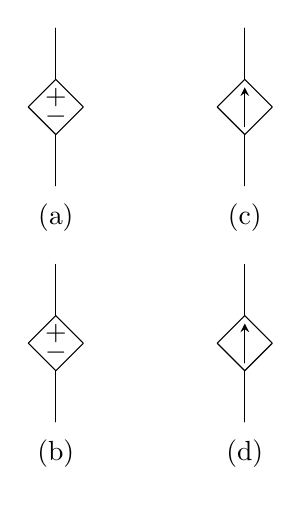
\begin{tikzpicture}[>=stealth,line cap=round,line join=round,scale=0.5]

        % (a)
        \begin{scope}[xshift=0cm,yshift=0cm]
          \draw (0,-2) -- (0,-0.7);
          \draw (0,0.7) -- (0,2);
          \draw (0,-0.7) -- (0.7,0) -- (0,0.7) -- (-0.7,0) -- cycle;
          \node at (0,0.25) {$+$};
          \node at (0,-0.25) {$-$};
          \node at (0,-2.8) {(a)};
        \end{scope}

        % (b)
        \begin{scope}[xshift=0cm,yshift=-6cm]
          \draw (0,-2) -- (0,-0.7);
          \draw (0,0.7) -- (0,2);
          \draw (0,-0.7) -- (0.7,0) -- (0,0.7) -- (-0.7,0) -- cycle;
          \node at (0,0.25) {$+$};
          \node at (0,-0.25) {$-$};
          \node at (0,-2.8) {(b)};
        \end{scope}

        % (c)
        \begin{scope}[xshift=4.8cm,yshift=0cm]
          \draw (0,-2) -- (0,-0.7);
          \draw (0,0.7) -- (0,2);
          \draw (0,-0.7) -- (0.7,0) -- (0,0.7) -- (-0.7,0) -- cycle;
          \draw[->] (0,-0.5) -- (0,0.5);
          \node at (0,-2.8) {(c)};
        \end{scope}

        % (d)
        \begin{scope}[xshift=4.8cm,yshift=-6cm]
          \draw (0,-2) -- (0,-0.7);
          \draw (0,0.7) -- (0,2);
          \draw (0,-0.7) -- (0.7,0) -- (0,0.7) -- (-0.7,0) -- cycle;
          \draw[->] (0,-0.5) -- (0,0.5);
          \node at (0,-2.8) {(d)};
        \end{scope}

      \end{tikzpicture}}
    \end{minipage}

  \item 控制量 $v_x$ 或 $i_x$ 通常在电路的其他支路,通过额外的标注给出。
\end{itemize}
\subsection{含受控源电路的求解思路}
\begin{enumerate}
  \item 像处理普通电路那样,先给所有电压、电流设参考方向。
  \item 对每个元件写元件方程:电阻用欧姆定律,独立源写出固定 $v$ 或 $i$。
  \item 对受控源,写出\textbf{控制关系}(如 $v = \mu v_x$),把 $v_x$ 或 $i_x$ 看作\mbox{未知量之一。}
  \item 用 KCL、KVL 列出足够多的方程,把受控源关系一起纳入方程组。
  \item 解方程得到所有未知电压、电流、控制量。
\end{enumerate}

\subsection{受控源的作用}
\begin{itemize}
  \item 是描述放大器、运算放大器、晶体管等\textbf{有源器件}的标准模型;
  \item 使线性电路中出现“输入–输出”关系,可以表达增益、反馈等概念;
  \item 在后续章节(放大电路、运放电路、滤波器等)会频繁出现。
\end{itemize}
\end{document}
